\documentclass[12pt,a4paper]{article}
\usepackage[utf8]{inputenc}
\usepackage[english,russian]{babel}
\usepackage{indentfirst}
\usepackage{misccorr}
\usepackage{graphicx}
\usepackage{amsmath}
\usepackage{parskip}
\usepackage[top=2cm, bottom=1cm, left=1cm, right=1cm]{geometry}
\usepackage[most]{tcolorbox}
\usepackage{hyperref}
\usepackage{fancyhdr}

\hypersetup{
	colorlinks,
	citecolor=black,
	filecolor=black,
	linkcolor=blue,
	urlcolor=blue
}

\pagestyle{fancy}
\lhead{Дифракция света на периодических структурах}
\rhead{\thepage}
\cfoot{}

\graphicspath{{pic/}, {~/Pictures/TeXImgs/}}

\newcommand{\sfrac}[2]{\dfrac{\strut #1}{\strut #2}}

\newcounter{picture}
\setcounter{picture}{1}
\newcounter{tbl}
\setcounter{tbl}{1}
\newcommand{\embed}[3]{\begin{center}
		\includegraphics[scale=#2]{#1}
		\\\textbf{Рис. \thepicture:} #3
		\label{pic_\thepicture}
		\addtocounter{picture}{1}
\end{center}}
\newcommand{\embedeps}[3]{\begin{center}
		\includegraphics[width=#2\linewidth]{#1}
		\\\textbf{Рис. \thepicture:} #3
		\label{pic_\thepicture}
		\addtocounter{picture}{1}
\end{center}}
\newcommand{\embedtbl}[3]{\begin{center}
		\begin{tabular}{#1}
			#2
		\end{tabular}
		\\\textbf{Табл. \thetbl:} #3
		\label{tbl_\thetbl}
		\addtocounter{tbl}{1}
\end{center}}
\newcommand{\picref}[1]{\hyperref[pic_#1]{Рис. #1}}
\newcommand{\tblref}[1]{\hyperref[tbl_#1]{Табл. #1}}

\begin{document}
	\begin{titlepage}
		\vspace*{\fill}
		
		\begin{center}
			
\includegraphics[scale=0.07]{MIPT_difr.png}
			\\[0.7cm]\Huge Московский Физико-Технический Институт\\(национальный исследовательский университет)
			\\[2cm]\LARGE Отчет по эксперименту
			\\[0.5cm]\noindent\rule{\textwidth}{1pt}
			\\\Huge\textbf{Дифракция света на периодических структурах}
			\\[-0.5cm]\noindent\rule{\textwidth}{1pt}
		\end{center}
		
		\begin{flushleft}
			\textit{Работа №4.3.6; дата: 08.04.23}\hfill\textit{Семестр: 4}
		\end{flushleft}
		
		\vspace*{\fill}
		
		\begin{flushleft}
			Выполнил: \hspace{\fill} Группа:
			\\Кошелев Александр \hspace{\fill} Б05-105
		\end{flushleft}
	\end{titlepage}
	
	\setcounter{page}{2}
	
	\section{Введение}
	
	\paragraph*{Цель работы:} \hfill
	
	Изучение явления саморепродукции и применение его к измерению параметров периодических структур.
	
	\paragraph*{В работе используются:} \hfill
	
	Лазер, кассета с сетками, мира, короткофокусная линза с микрометрическим винтом, экран, линейка.
	
	\paragraph*{Схема установки:} \hfill
	
	Хорошим приближением к плоской волне в нашем эксперименте является излучение лазера.
	
	\embed{PIC_1.png}{0.3}{Схема установки}
	
	Луч лазера падает перпендикулярно на периодический объект $O$, установленный в	плоскости $P_0$.
	За плоскостью $P_0$ (в плоскостях $P_1$ -- $P_N$  ) периодически по $z$ возникают изображения объекта, которые с помощью линзы Л можно поочерёдно проецировать на экран, установленный в плоскости Э. Если убрать линзу, то на экране наблюдается картина дифракции луча лазера на периодическом объекте.
	
	\section{Теоретическая справка}
	
	Экран устанавливается достаточно далеко от объекта, так что продифрагировавшие лучи, соответствующие различным порядкам дифракции ($\sin \theta_n = n\lambda/d$), разделяются.
	
	Измерив расстояние между дифракционными максимумами и расстояние от объекта до экрана, мы определим $\sin \theta_n$ и $d$.
	
	В нашей работе в качестве периодических объектов применяется «мира» -- набор различным образом ориентированных одномерных решёток разного периода, а также	двумерная решётка-сетка.
	
	\embed{PIC_2.png}{0.3}{Спектр решетки-сетки}
	
	Сетку можно рассматривать как две взаимно перпендикулярные решётки. Узкий пучок монохроматического света, пройдя через первую решётку с вертикальными штрихами, должен дать совокупность максимумов, расположенных вдоль горизонтальной линии. Световой пучок, соответствующий каждому максимуму, проходя через вторую решётку, распадается на новую совокупность пучков, дающих максимумы вдоль вертикальной линии. В результате главные максимумы возникают тогда, когда одновременно выполняются условия
	
	$$d \sin \theta_x = m_x \lambda \ \ \ \ \ \ \ \ \ d \sin \theta_y = m_y \lambda$$
	
	где $m_x$ и $m_y$ -- два целых числа, характеризующих порядки дифракционных максимумов, $\theta_x$ и $\theta_y$ -- направления на главные дифракционные максимумы в горизонтальной и вертикальной плоскостях соответственно. Максимумы показаны кружками, размеры которых характеризуют интенсивность.
	
	\section{Ход работы}
	
	\subsection{Определение периода решеток по их пространственному спектру}
	
	Соберем установку без линзы и пронаблюдаем дифракционные картины на различных решетках.
	
	\begin{figure}[h]
		\begin{minipage}{0.33\linewidth}
			\begin{center}
				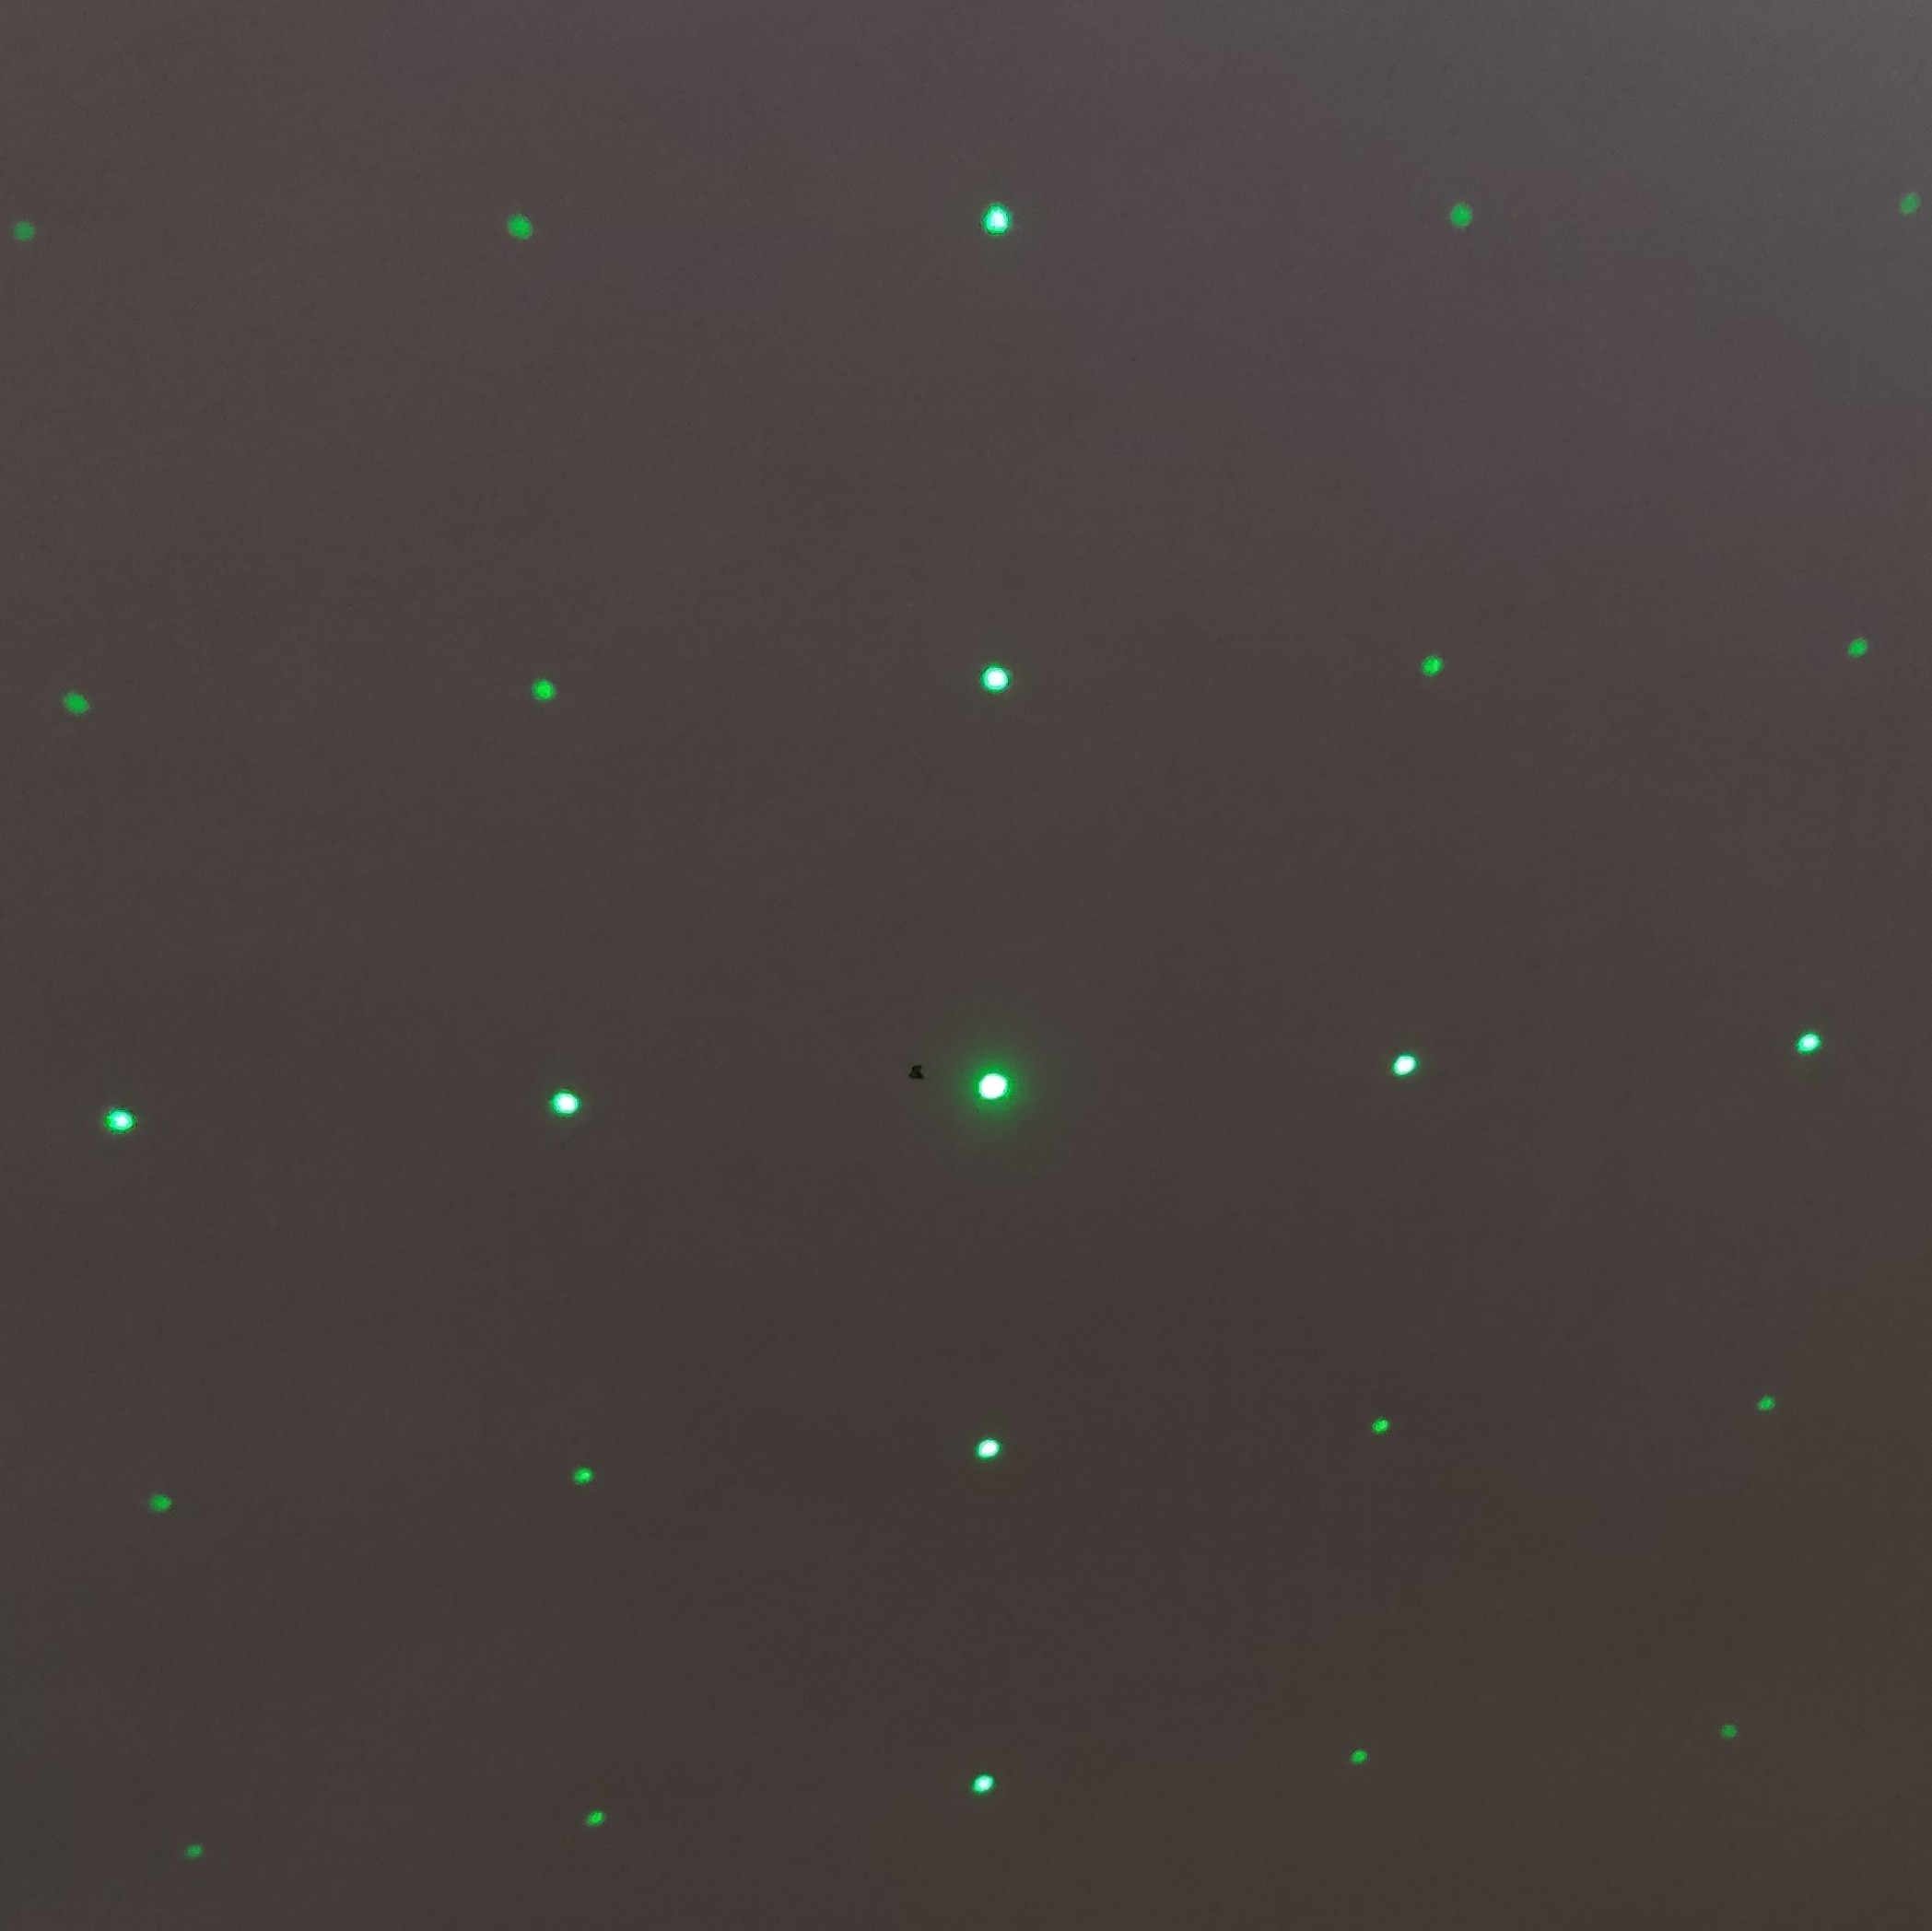
\includegraphics[width=4cm]{PIC_3_1.jpg}
				\\1
			\end{center}
		\end{minipage}
		\begin{minipage}{0.33\linewidth}
			\begin{center}
				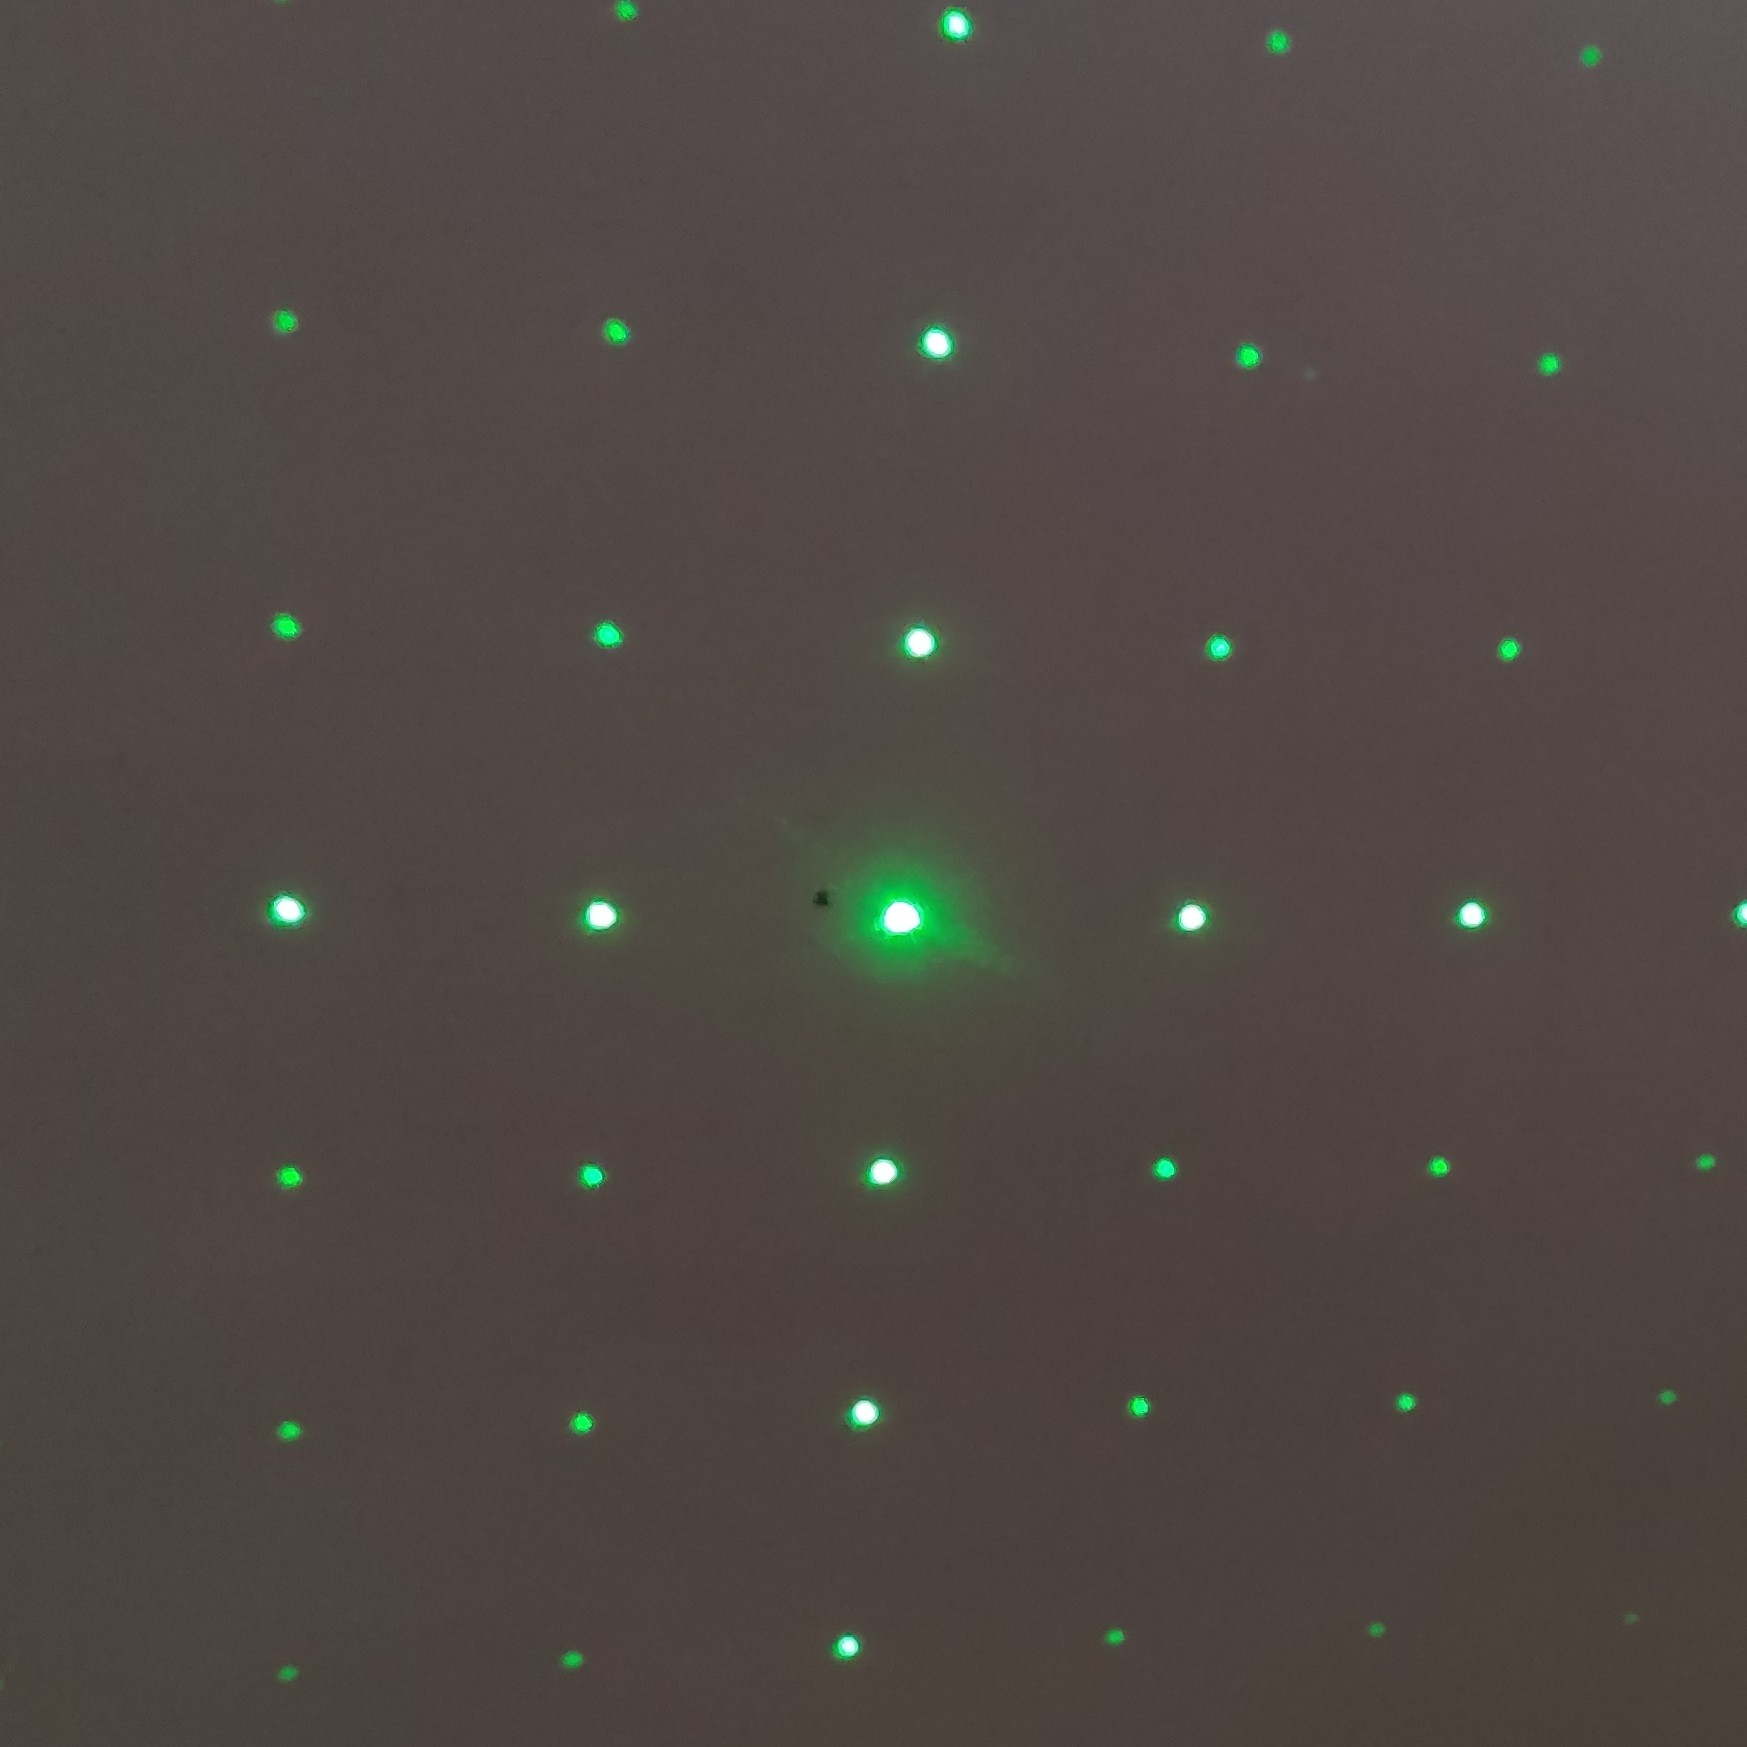
\includegraphics[width=4cm]{PIC_3_2.jpg}
				\\2
			\end{center}
		\end{minipage}
		\begin{minipage}{0.33\linewidth}
			\begin{center}
				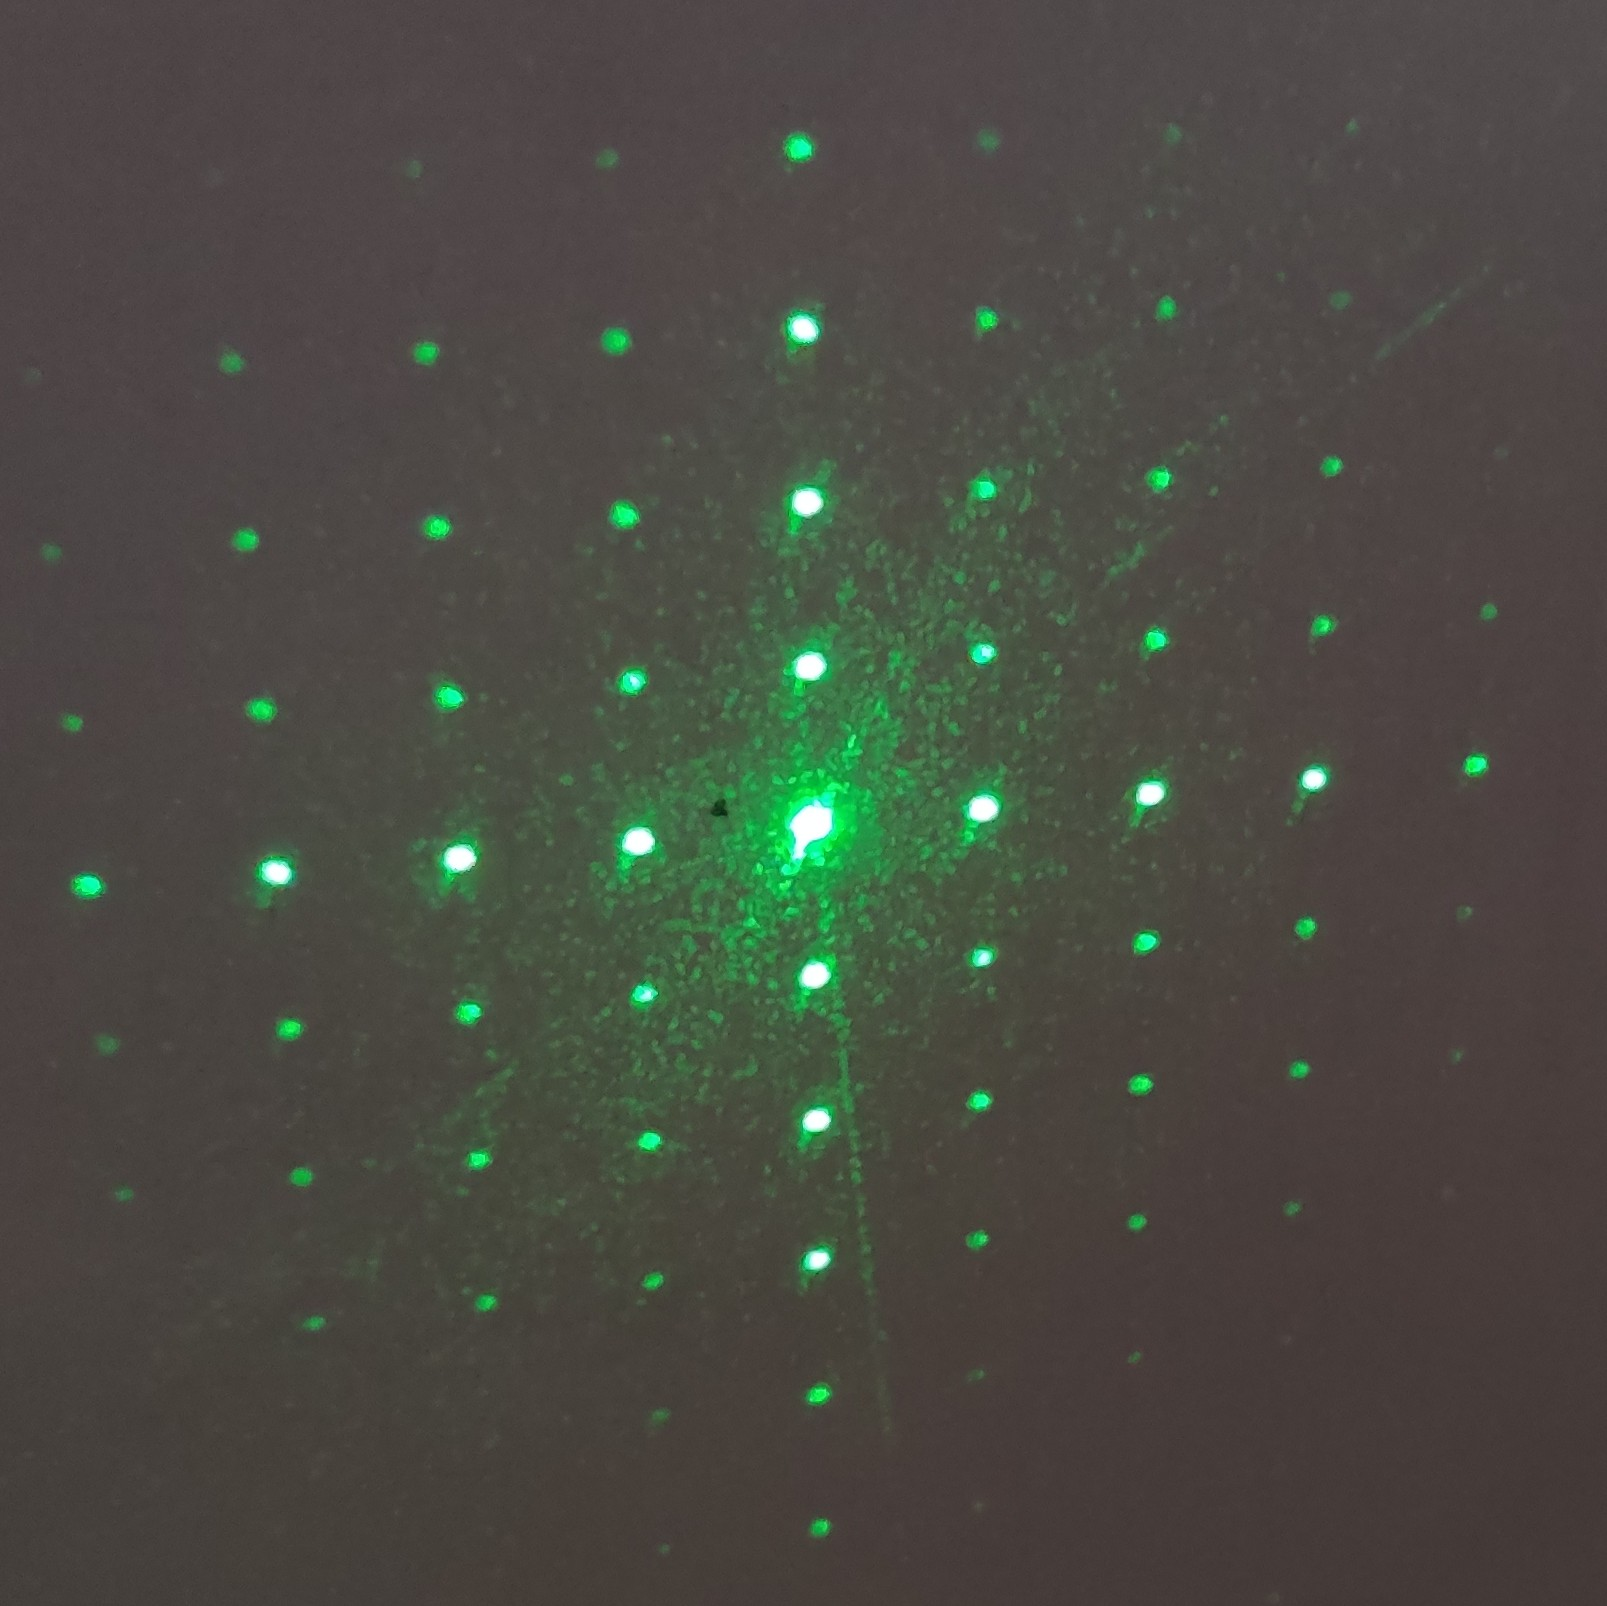
\includegraphics[width=4cm]{PIC_3_3.jpg}
				\\3
			\end{center}
		\end{minipage}
	\end{figure}
	\begin{figure}[h]
		\begin{minipage}{0.5\linewidth}
			\begin{center}
				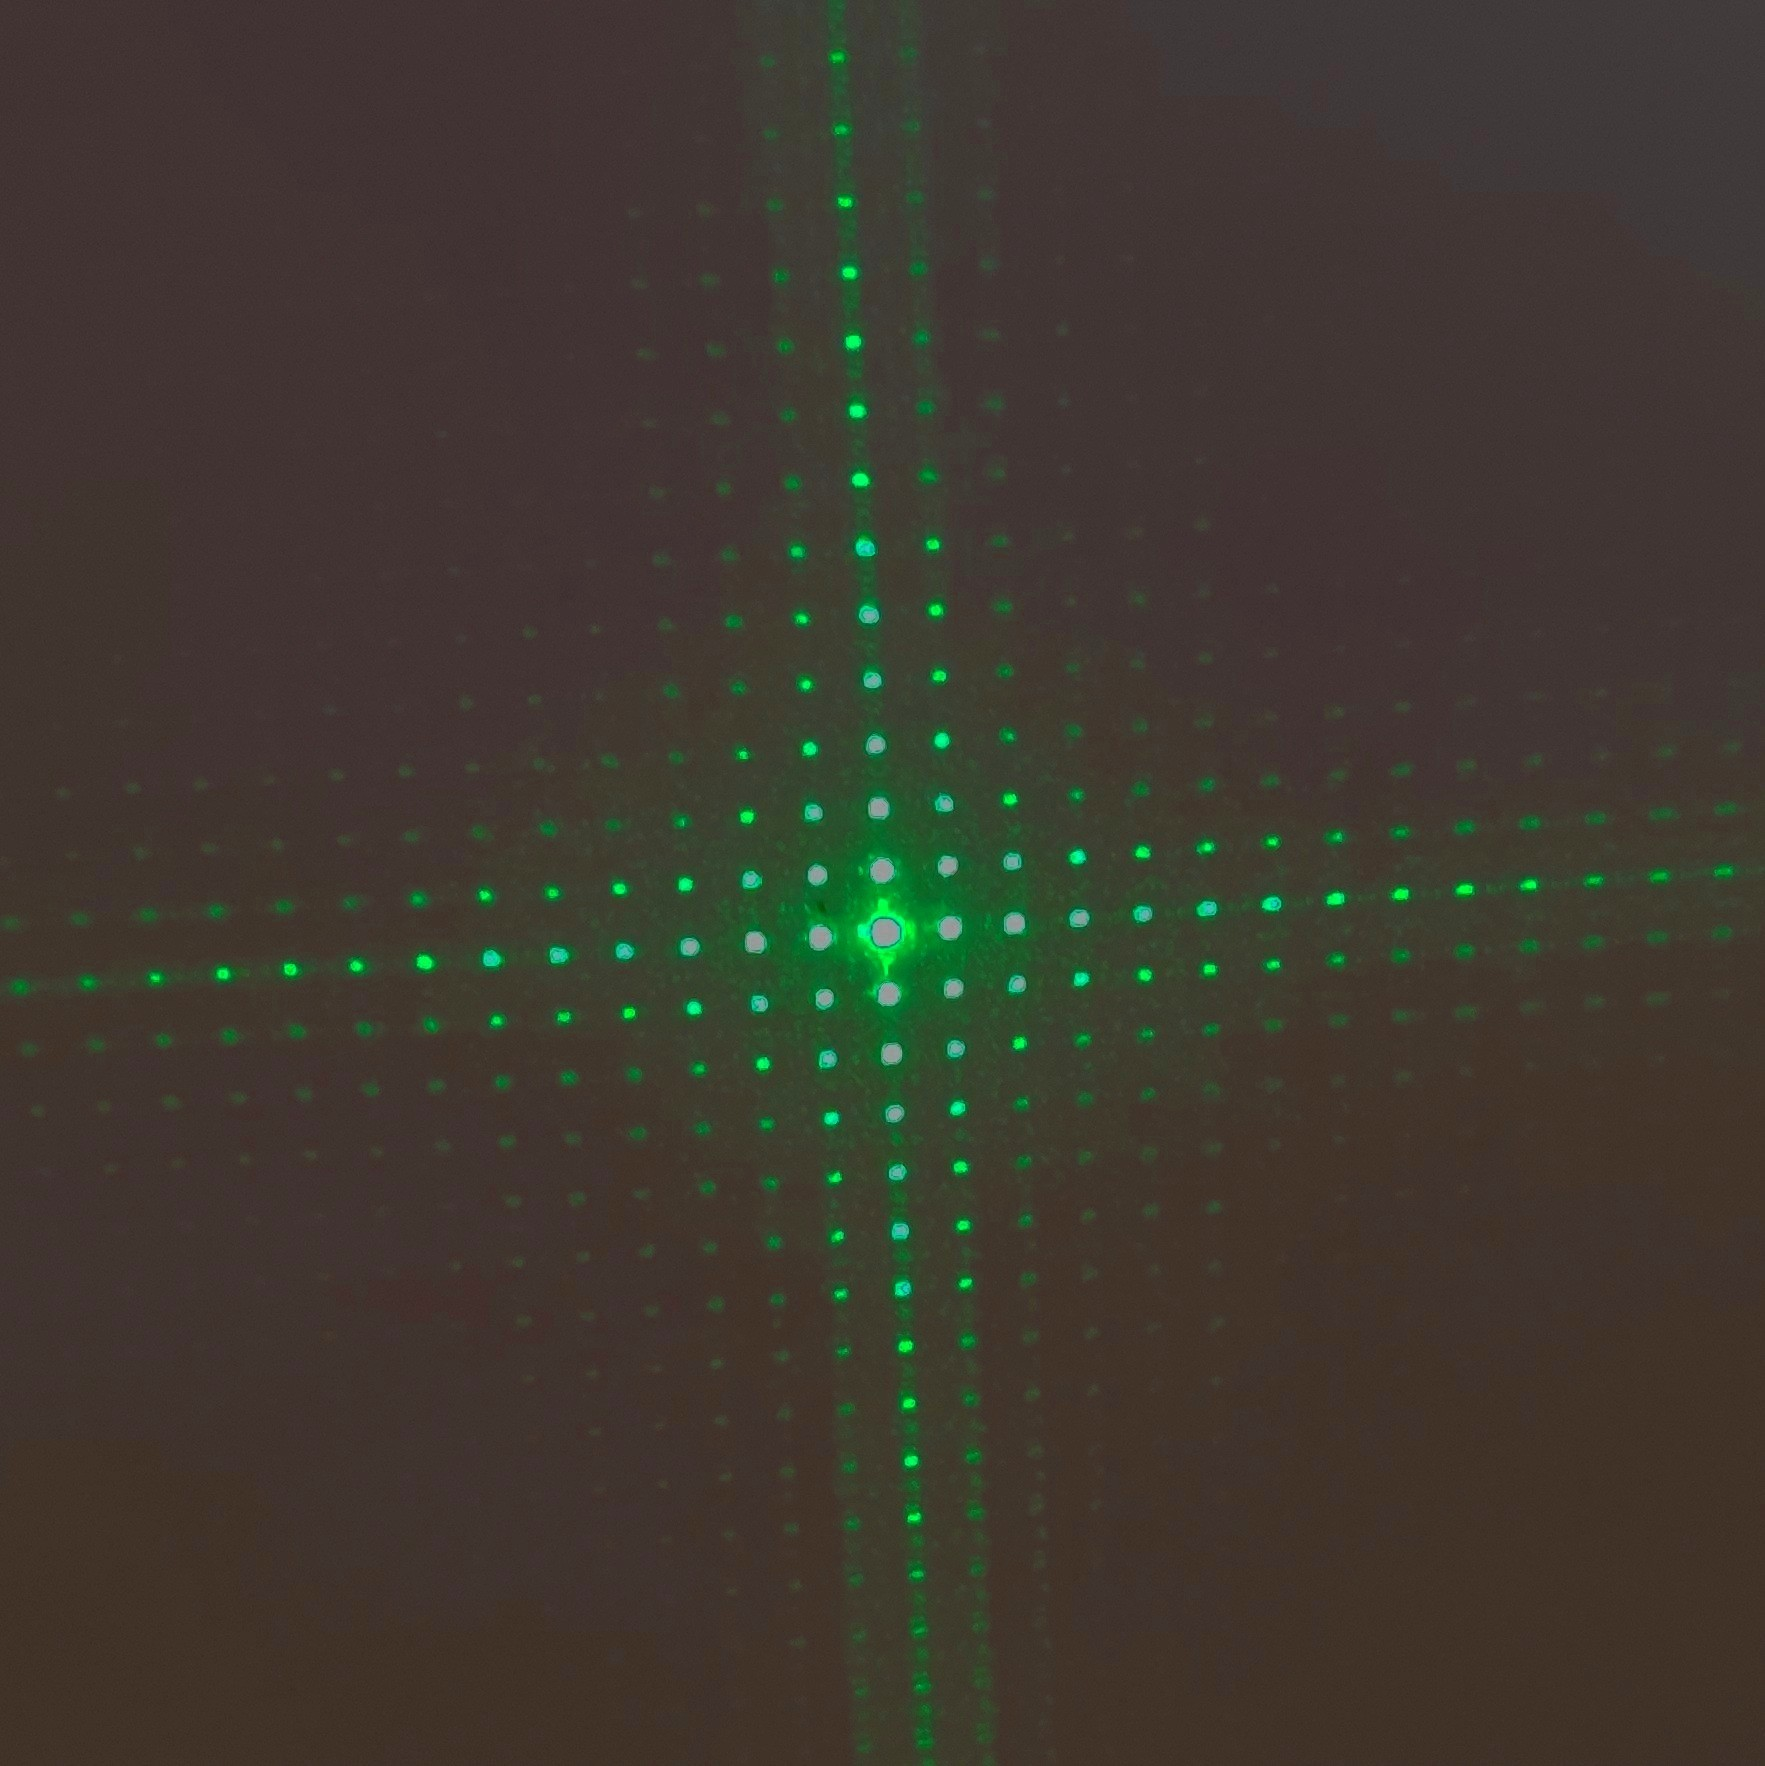
\includegraphics[width=4cm]{PIC_3_4.jpg}
				\\4
			\end{center}
		\end{minipage}
		\begin{minipage}{0.5\linewidth}
			\begin{center}
				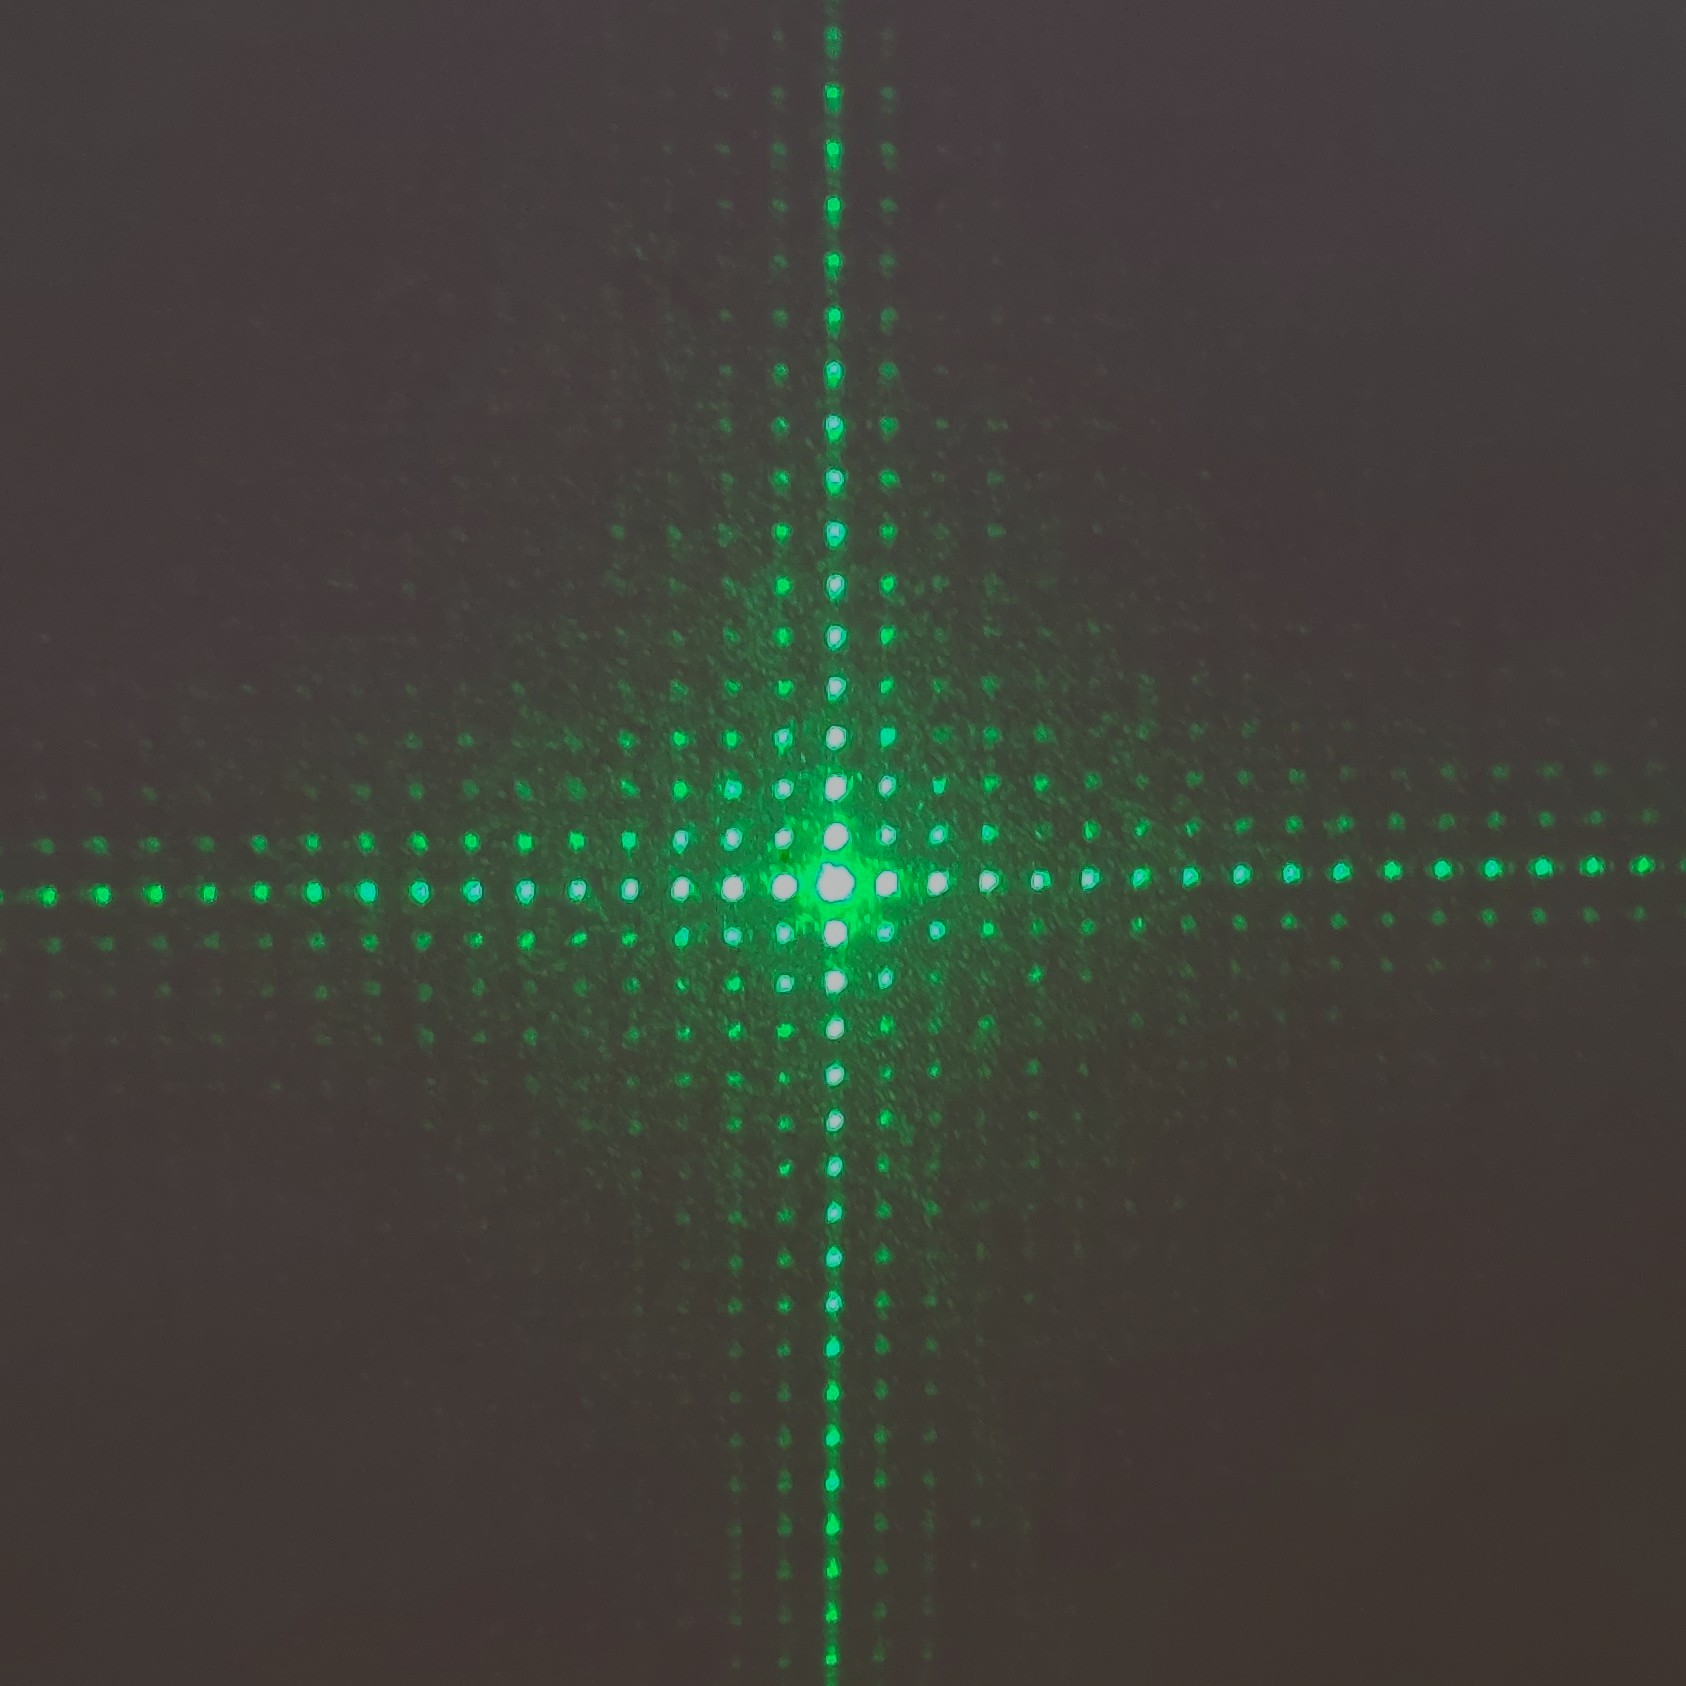
\includegraphics[width=4cm]{PIC_3_5.jpg}
				\\5
			\end{center}
		\end{minipage}
	\begin{center}
		\textbf{Рис. \thepicture:} Дифракционные картины в решетках по номеру
		\label{pic_\thepicture}
		\addtocounter{picture}{1}
	\end{center}
	\end{figure}
	
	Измерим расстояния между максимумами для разных решеток:
	
	\embedtbl{|c||c|c|c|c|c|}{
		\hline
		$i$, \#  & 1 & 2 & 3 & 4 & 5
		\\\hline
		$x$, мм & $31.0 \pm 0.5$ & $24.0 \pm 0.5$ & $12 \pm 0.5$ & $6.5 \pm 0.5$ & $4.5 \pm 0.5$
		\\\hline
	}{Расстояния между максимумами}
	
	Непосредственно по этим картинам рассчитаем периоды сооответствующих решеток (при $L = 136.3$ см, $\lambda = 532$ нм):
	
	$$d = \sfrac{\lambda L}{x}$$
	
	\embedtbl{|c||c|c|c|c|c|}{
		\hline
		$i$, \# & 1 & 2 & 3 & 4 & 5
		\\\hline
		$d$, мм & 0.023 $\pm$ 0.001 & 0.030 $\pm$ 0.001 & 0.060 $\pm$ 0.003 & 0.112 $\pm$ 0.009 & 0.161 $\pm$ 0.018
		\\\hline
	}{Периоды решеток}

	\subsection{Определение периода решеток по увеличенному изображению}
	
	Соберем установку с линзой и пронаблюдаем увеличенные изображения решеток.
	
	\begin{figure}[h]
		\begin{minipage}{0.33\linewidth}
			\begin{center}
				
\includegraphics[width=4cm]{PIC_4_1.jpg}
				\\1
			\end{center}
		\end{minipage}
		\begin{minipage}{0.33\linewidth}
			\begin{center}
				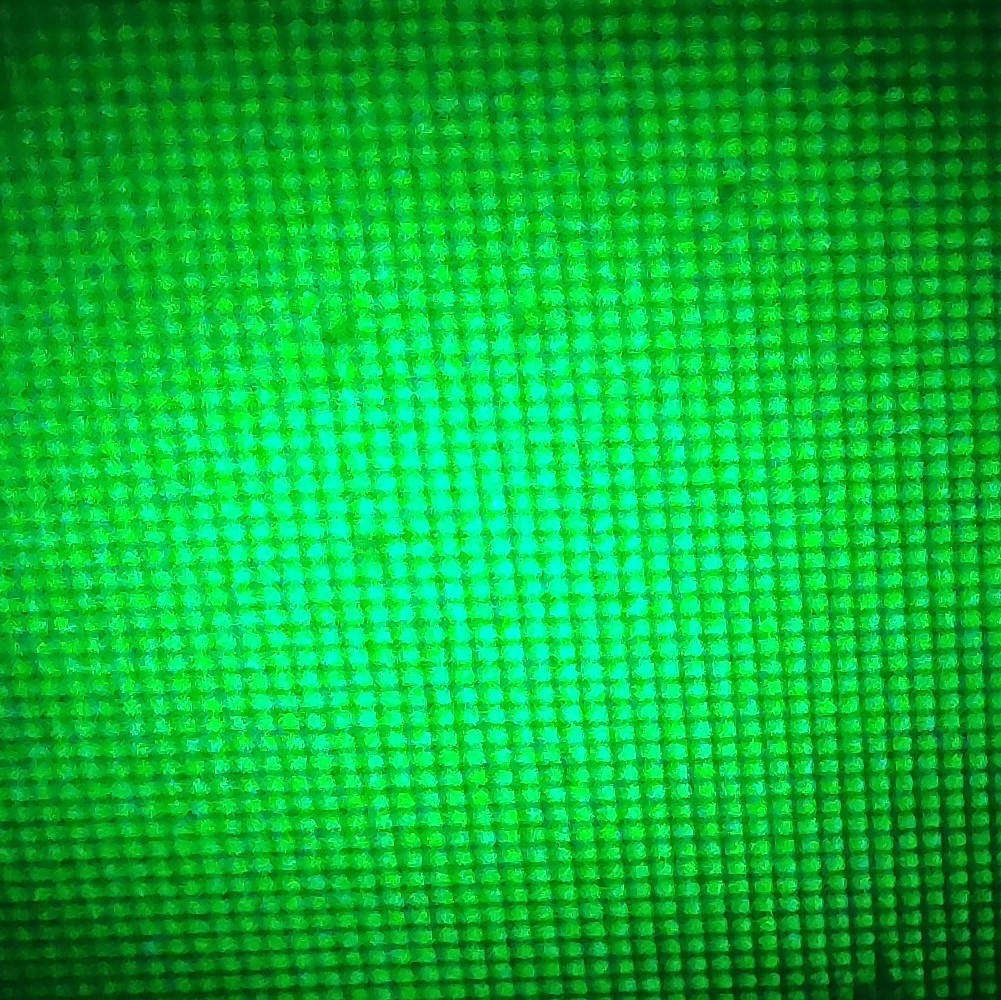
\includegraphics[width=4cm]{PIC_4_2.jpg}
				\\2
			\end{center}
		\end{minipage}
		\begin{minipage}{0.33\linewidth}
			\begin{center}
				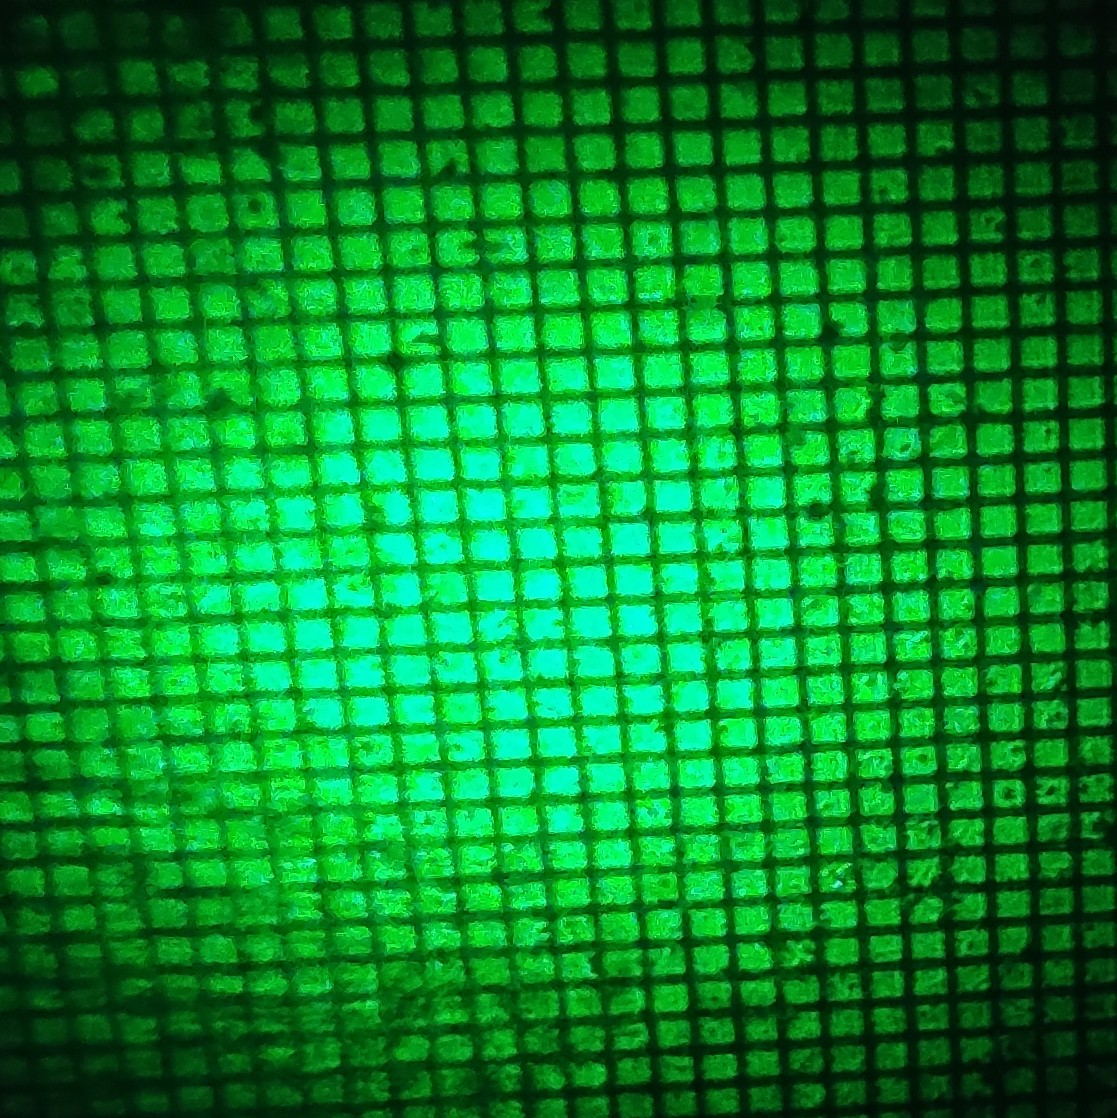
\includegraphics[width=4cm]{PIC_4_3.jpg}
				\\3
			\end{center}
		\end{minipage}
	\end{figure}
	\begin{figure}[h]
		\begin{minipage}{0.5\linewidth}
			\begin{center}
				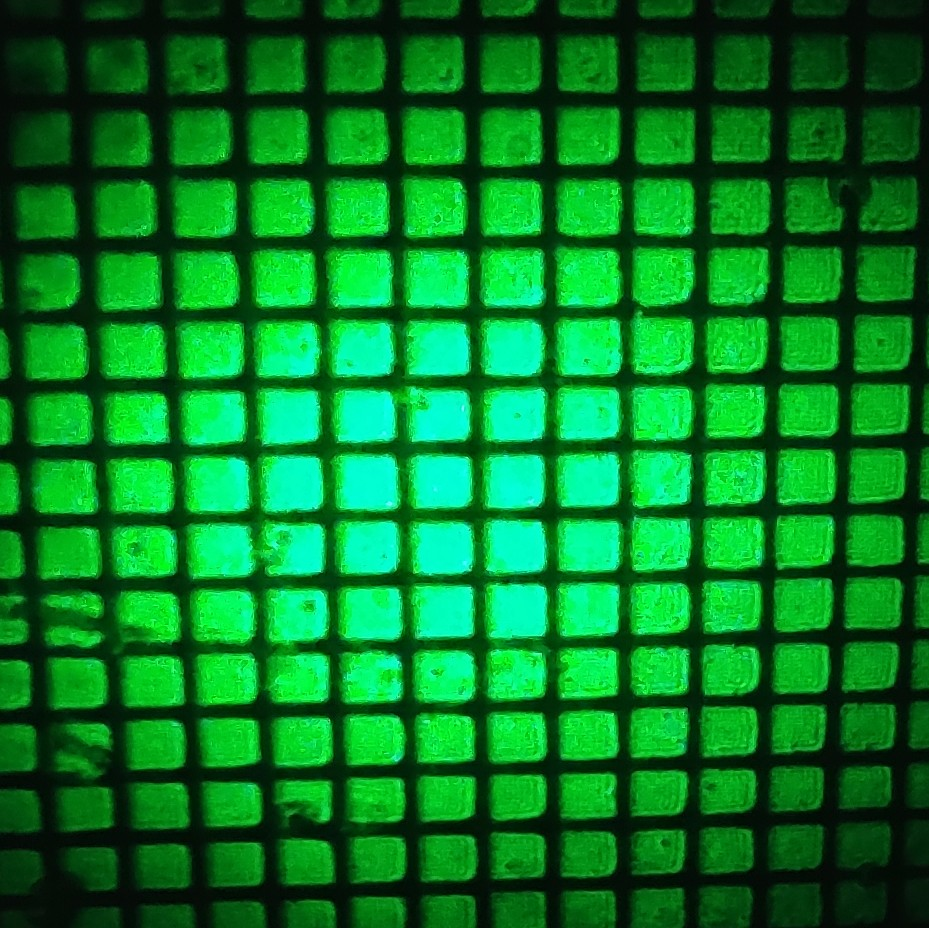
\includegraphics[width=4cm]{PIC_4_4.jpg}
				\\4
			\end{center}
		\end{minipage}
		\begin{minipage}{0.5\linewidth}
			\begin{center}
				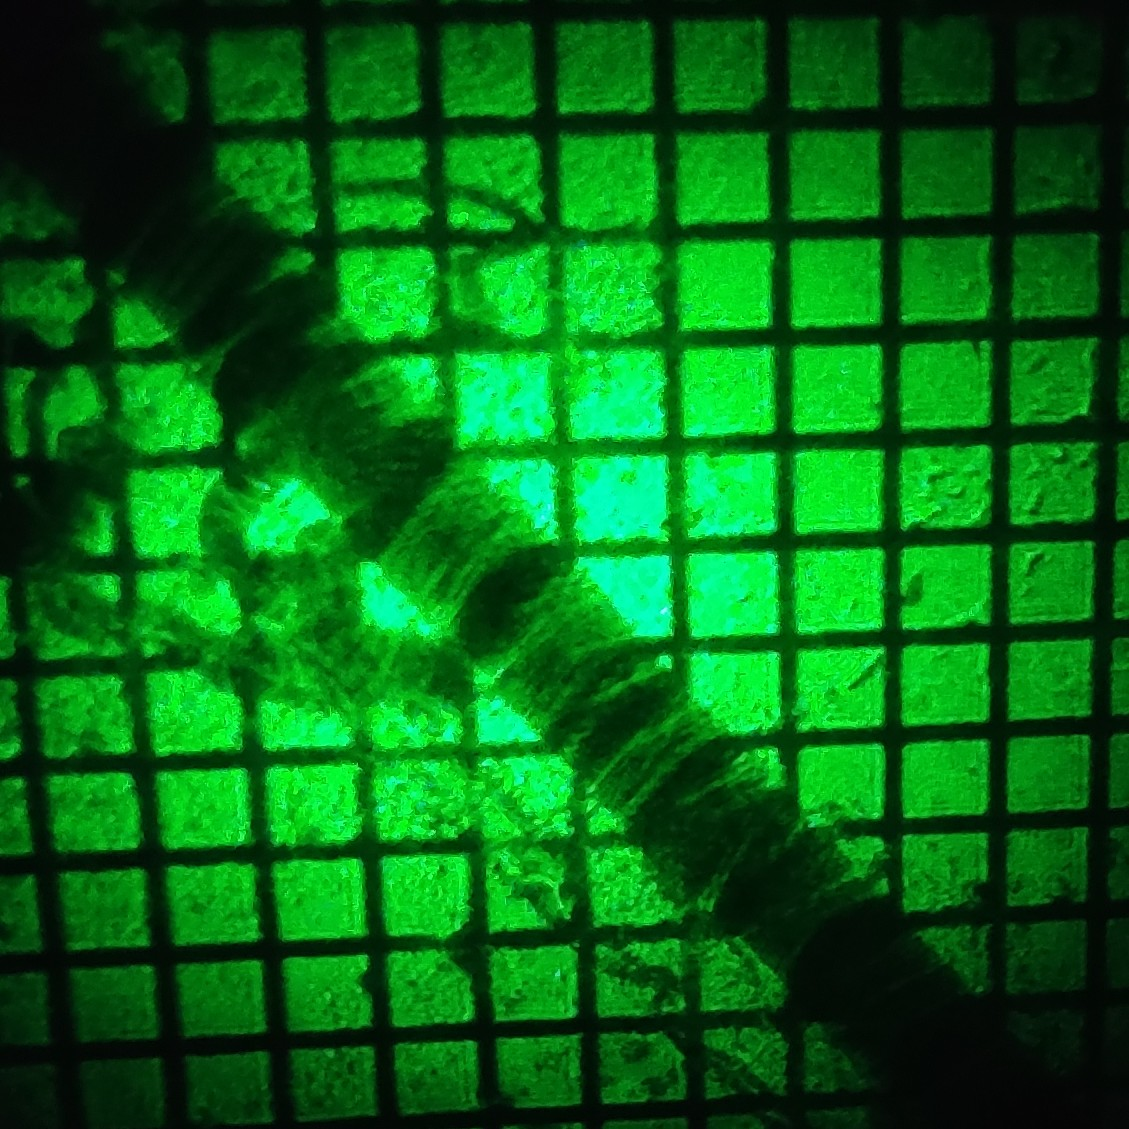
\includegraphics[width=4cm]{PIC_4_5.jpg}
				\\5
			\end{center}
		\end{minipage}
		\begin{center}
			\textbf{Рис. \thepicture:} Увеличенные изображения решеток по номеру
			\label{pic_\thepicture}
			\addtocounter{picture}{1}
		\end{center}
	\end{figure}
	
	Определим размеры клеток, полученных с помощью линзы, на экране (рассматриваем геометрическое изображение решётки) ($D$). Расстояние от линзы до сетки $a$, от линзы до экрана $b$, тогда период сетки считается по формуле:
	
	$$d = D\frac{a}{b}$$
	
	Результаты измерения периода занесём в таблицу (при $a = 5.5$ см, $b = 127.6$ см):

	\embedtbl{|c||c|c|c|c|c|}{
		\hline
		$i$, \# & 1 & 2 & 3 & 4 & 5
		\\\hline
		$d$, мм & 0.022 $\pm$ 0.005 & 0.043 $\pm$ 0.006 & 0.065 $\pm$ 0.007 & 0.129 $\pm$ 0.013 & 0.172 $\pm$ 0.016
		\\\hline
	}{Периоды решеток}
	
	\subsection{Исследование эффекта саморепродукции с помощью решеток}
	
	Будем передвигать линзу и пронаблюдаем эффект саморепродукции на примере решетки 4.
	
	\newpage
	
	\begin{figure}[h]
		\begin{minipage}{0.33\linewidth}
			\begin{center}
				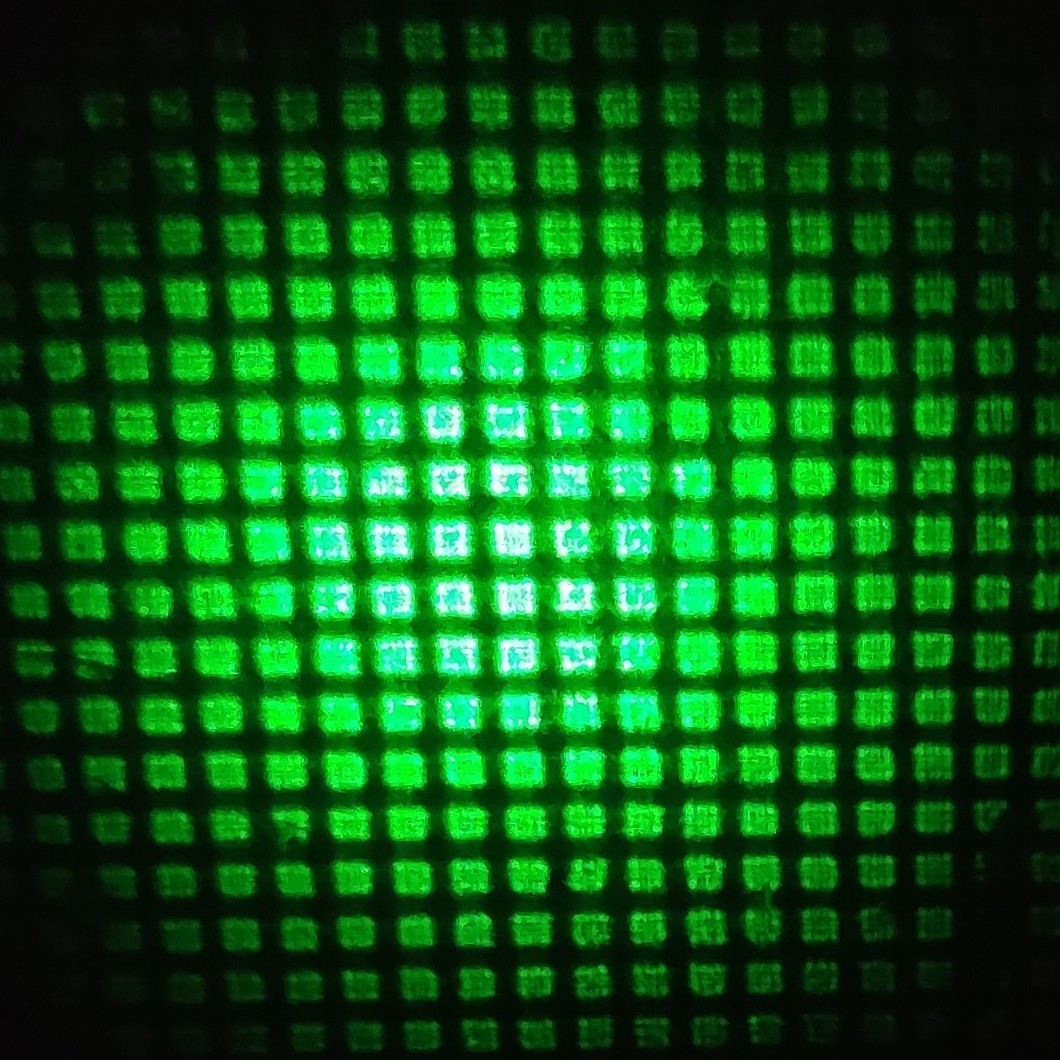
\includegraphics[width=4cm]{PIC_5_0.jpg}
				\\0
			\end{center}
		\end{minipage}
		\begin{minipage}{0.33\linewidth}
			\begin{center}
				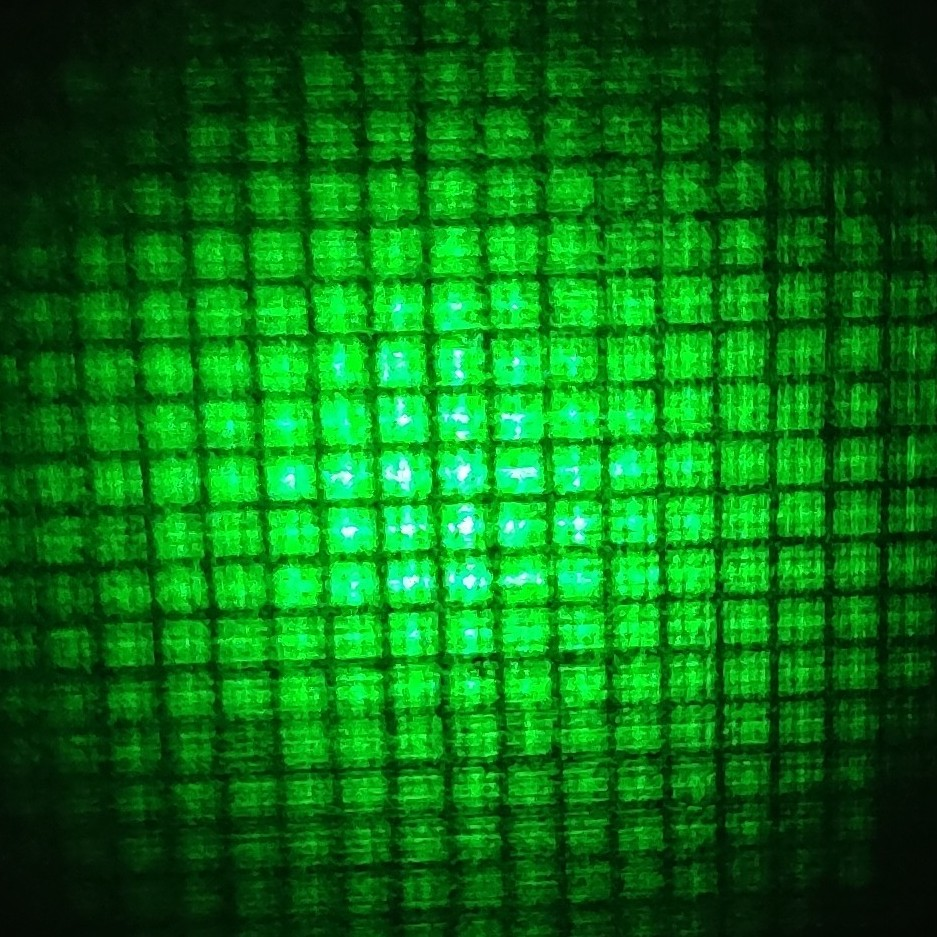
\includegraphics[width=4cm]{PIC_5_1.jpg}
				\\1
			\end{center}
		\end{minipage}
		\begin{minipage}{0.33\linewidth}
			\begin{center}
				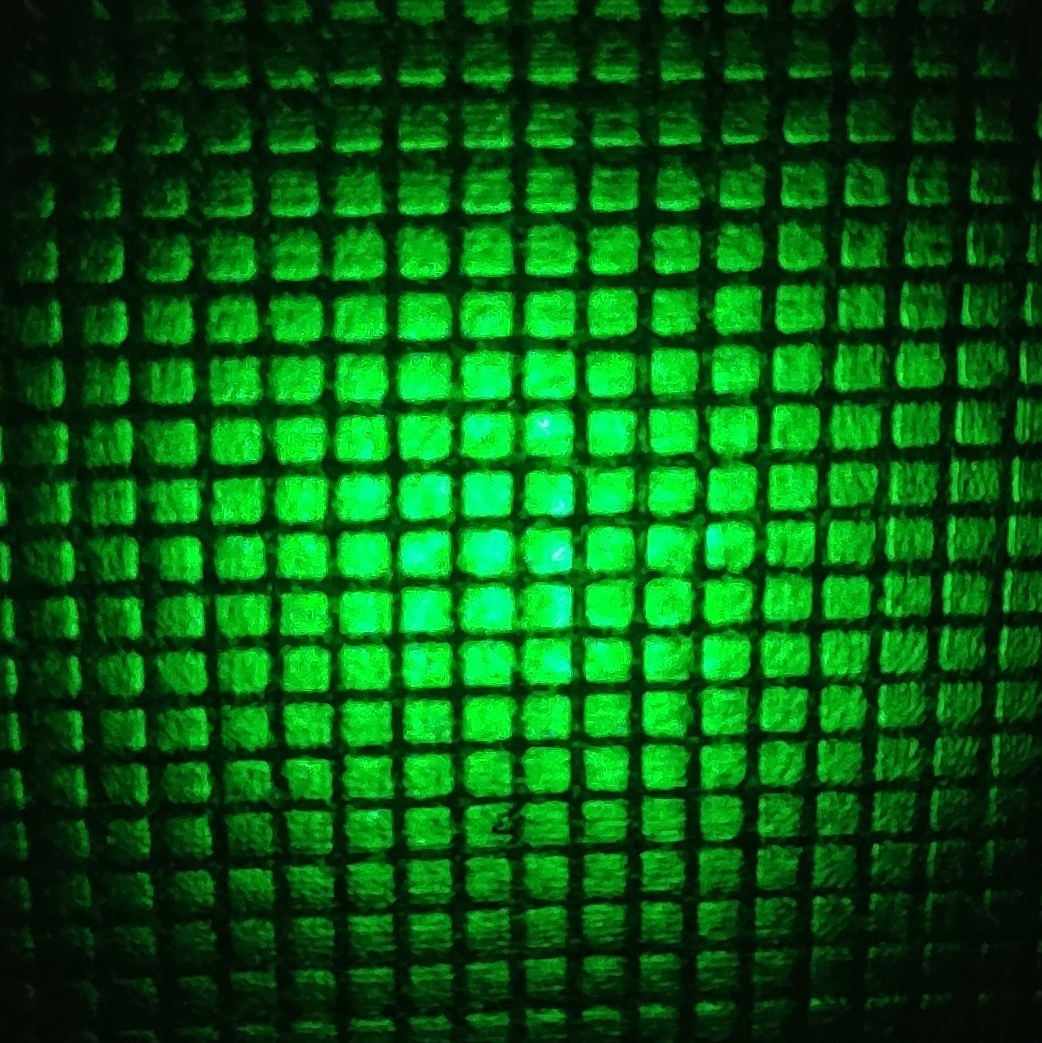
\includegraphics[width=4cm]{PIC_5_2.jpg}
				\\2
			\end{center}
		\end{minipage}
	\end{figure}
	\begin{figure}[h]
		\begin{minipage}{0.5\linewidth}
			\begin{center}
				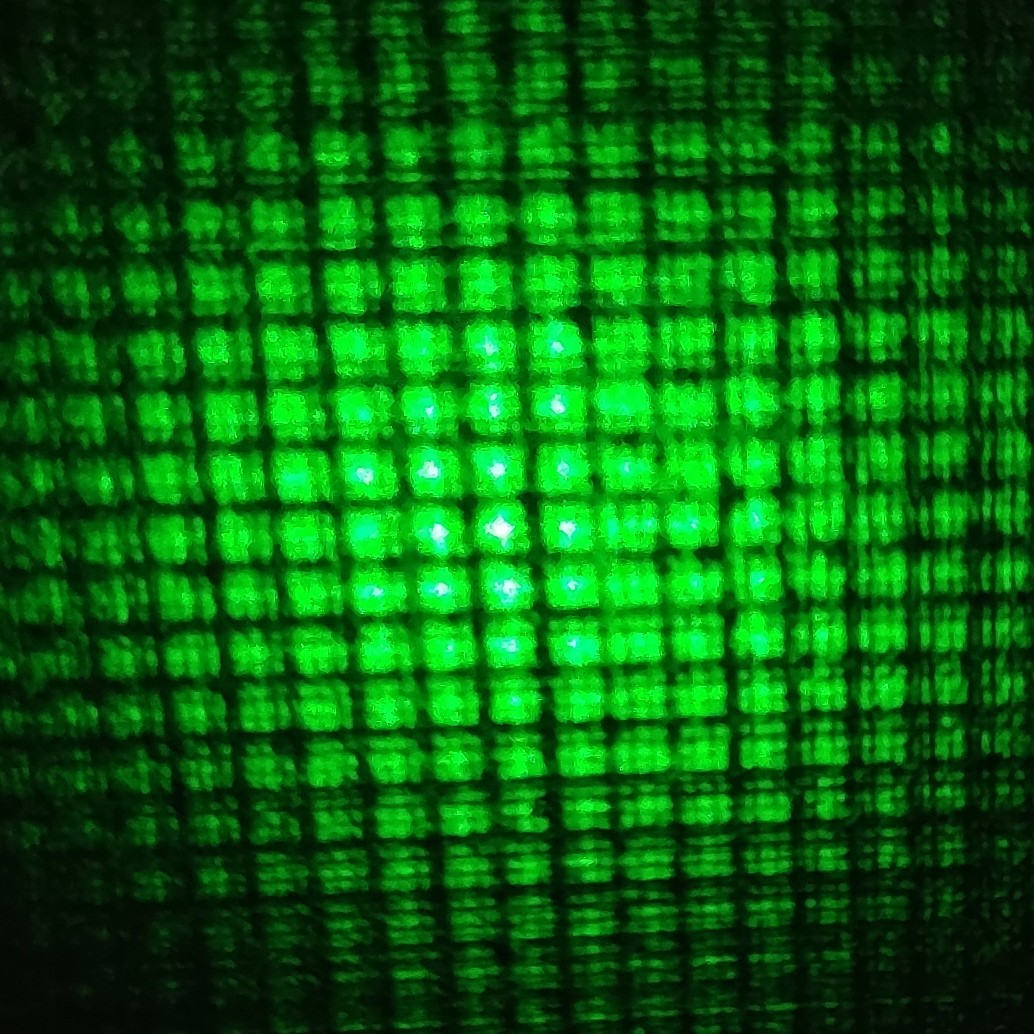
\includegraphics[width=4cm]{PIC_5_3.jpg}
				\\3
			\end{center}
		\end{minipage}
		\begin{minipage}{0.5\linewidth}
			\begin{center}
				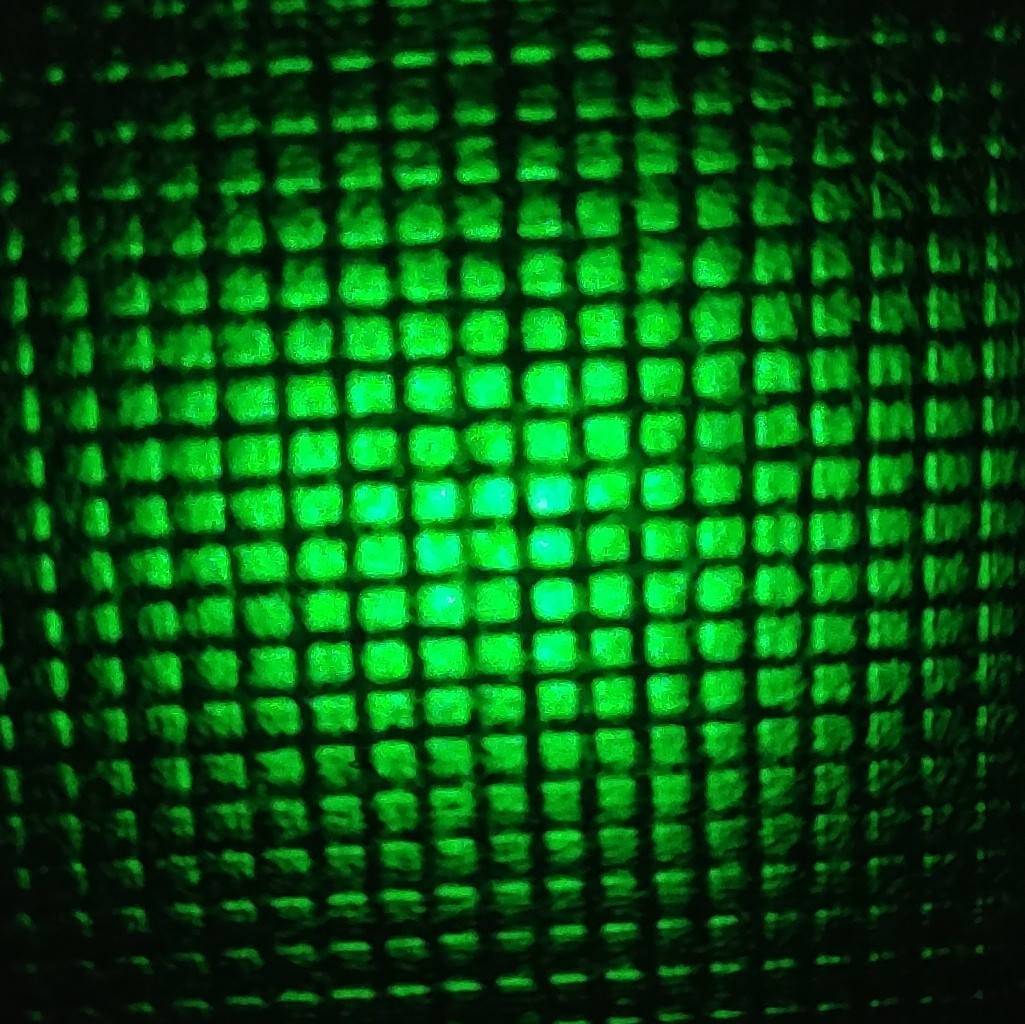
\includegraphics[width=4cm]{PIC_5_4.jpg}
				\\4
			\end{center}
		\end{minipage}
		\begin{center}
			\textbf{Рис. \thepicture:} Плоскости репродукции по номеру
			\label{pic_\thepicture}
			\addtocounter{picture}{1}
		\end{center}
	\end{figure}
	
	Найдём координаты  $z_n$ плоскостей саморепродукции, построим график $z_n=f(n)$, по коэффициенту наклона графика $\gamma$ определим период решётки:
	\begin{equation}
		d = \sqrt{\frac{\gamma \lambda}{2}}        
	\end{equation}
	
	\embedeps{PIC_6.eps}{0.7}{График зависимости $z_n$ для решетки 1}
	\embedeps{PIC_7.eps}{0.7}{График зависимости $z_n$ для решетки 2}
	\embedeps{PIC_8.eps}{0.7}{График зависимости $z_n$ для решетки 3}
	\embedeps{PIC_9.eps}{0.7}{График зависимости $z_n$ для решетки 4}
	\embedeps{PIC_10.eps}{0.7}{График зависимости $z_n$ для решетки 5}
	
	\embedtbl{|c|c|c|c|c|c|}{
		\hline
		$i$, \# & 1 & 2 & 3 & 4 & 5
		\\\hline
		$\gamma$, cм & 0.056 $\pm$ 0.003 & 0.191 $\pm$ 0.012 & 0.357 $\pm$ 0.011 & 1.319 $\pm$ 0.053 & 2.480 $\pm$ 0.320
		\\\hline
		$d$, мм & 0.024 $\pm$ 0.012 & 0.045 $\pm$ 0.013 & 0.062 $\pm$ 0.009 & 0.118 $\pm$ 0.010 & 0.162 $\pm$ 0.019
		\\\hline
		
	}{Вычисление периода решетки}

	\subsection{Сравнение периодов решеток}
	
	Занесем полученные разными методами значения периодов решеток в одну таблицу для сравнения:
	
	\embedtbl{|c|c|c|c|c|c|}{
		\hline
		$d_{\text{спектр}}$, мм & 0.023 $\pm$ 0.001 & 0.030 $\pm$ 0.001 & 0.060 $\pm$ 0.003 & 0.112 $\pm$ 0.009 & 0.161 $\pm$ 0.018
		\\\hline
		$d_{\text{увел}}$, мм & 0.022 $\pm$ 0.005 & 0.043 $\pm$ 0.006 & 0.065 $\pm$ 0.007 & 0.129 $\pm$ 0.013 & 0.172 $\pm$ 0.016
		\\\hline
		$d_{\text{репрод}}$, мм & 0.024 $\pm$ 0.012 & 0.045 $\pm$ 0.013 & 0.062 $\pm$ 0.009 & 0.118 $\pm$ 0.010 & 0.162 $\pm$ 0.019
		\\\hline
	}{Сравнение полученных периодов}

	Из данной таблицы видно, что полученные периоды совпадают в пределах погрешности. Наиболее точным выглядит метод исследования увеличенного изображения.
	
	\subsection{Исследование решеток миры}
	
	Рассмотрим решетки миры.
	
	\begin{figure}[h]
		\begin{minipage}{0.5\linewidth}
			\begin{center}
				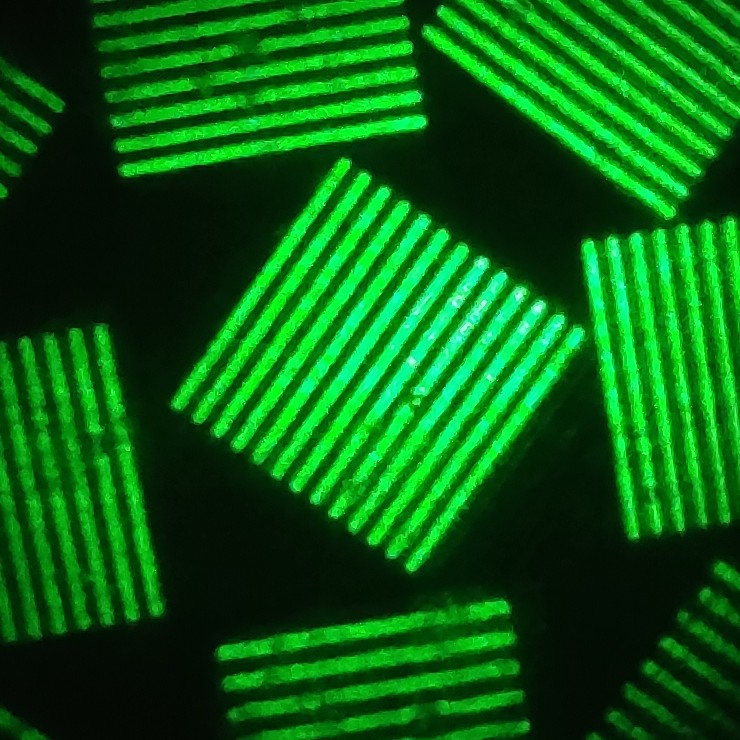
\includegraphics[width=5cm]{PIC_13_1.jpg}
				\\20
			\end{center}
		\end{minipage}
		\begin{minipage}{0.5\linewidth}
			\begin{center}
				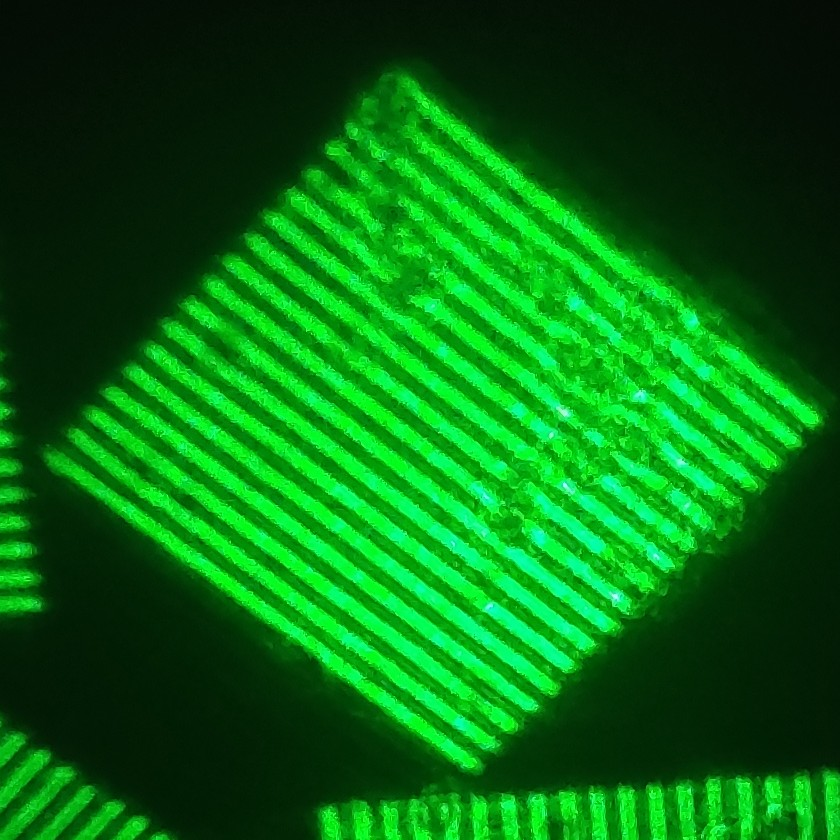
\includegraphics[width=5cm]{PIC_13_2.jpg}
				\\25
			\end{center}
		\end{minipage}
		\begin{center}
			\textbf{Рис. \thepicture:} Геометрические изображения решеток миры
			\label{pic_\thepicture}
			\addtocounter{picture}{1}
		\end{center}
	\end{figure}
	
	\embedeps{PIC_11.eps}{0.7}{График зависимости $z_n$ для миры 20}
	\embedeps{PIC_12.eps}{0.7}{График зависимости $z_n$ для миры 25}
	
	\embedtbl{|c|c|c|}{
		\hline
		$i$, \# & 20 & 25
		\\\hline
		$\gamma$, cм & 0.204 $\pm$ 0.018 & 0.296 $\pm$ 0.028
		\\\hline
		$d$, мм & 0.023 $\pm$ 0.008 & 0.028 $\pm$ 0.008
		\\\hline
	}{Исследование решеток миры}
	
	
	\section{Выводы}
	
	\begin{itemize}
		\item В работе исследованы 5 дифракционных решеток тремя различными способами, диаметры занесены в \tblref{5}.
		
		\item Значения, полученные методами изучения дифракционной картины, изучения увеличенного изображения и определения плоскостей саморепродукции совпадают в пределах погрешности.
		
		\item В работе также исследованы 2 решетки миры с известными параметрами, периоды занесены в \tblref{6}.
		
		\item Значения, полученные методом определения плоскостей саморепродукции, совпадают с известными в пределах погрешности.
	\end{itemize}
		
\end{document}